\paragraph{QuizziPedia::Front-End::Directives::EliminationAndModifyDirective}
\begin{figure} [ht]
	\centering
	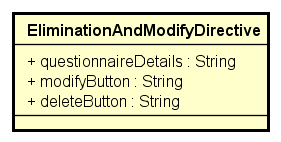
\includegraphics[scale=0.45]{UML/Classi/Front-End/QuizziPedia_Front-end_EliminationAndModifyDirective.png}
	\caption{QuizziPedia::Front-End::Views:EliminationAndModifyDirective}
\end{figure} \FloatBarrier
\begin{itemize}
	\item \textbf{Descrizione}: componente grafico contenente i bottoni per eliminare o modificare un questionario;
	\item \textbf{Utilizzo}: permette di eliminare un questionario o di modificarne uno esistente;
	\item \textbf{Relazioni con altre classi}:
	\begin{itemize}
		\item \textit{IN} \texttt{QuizEventModelView}: classe di tipo modelview la cui istanzazione è contenuta all'interno della variabile di ambiente \$scope di \texttt{Angular.js}. All'interno di essa sono presenti le variabili e i metodi necessari per il \textit{Two-Way Data-Binding\ped{G}} tra la view \texttt{QuizEventView} e il controller \texttt{QuizEventController};
		\item \textit{IN} \texttt{QuestionnaireManagementView}: view principale per la gestione dei questionari; 
		\item \textit{IN} \texttt{LangModel}: rappresenta il modello delle informazioni per la giusta traduzione dell'applicazione.
	\end{itemize}
	\item \textbf{Attributi}:
	\begin{itemize}
		\item {+ modifyButton: String} \\ Attributo che viene utilizzato per visualizzare la giusta traduzione della \textit{label\ped{G}} per il bottone di modifica del questionario selezionato, in italiano o in inglese; 
		\item {+ deleteButton: String} \\ Attributo che viene utilizzato per visualizzare la giusta traduzione della \textit{label\ped{G}} per il bottone di eliminazione del questionario selezionato, in italiano o in inglese.
	\end{itemize}
\end{itemize}

\paragraph{QuizziPedia::Front-End::Directives::ExamModalityDirective}
\begin{figure} [ht]
	\centering
	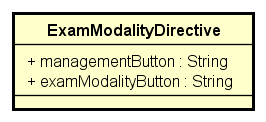
\includegraphics[scale=0.45]{UML/Classi/Front-End/QuizziPedia_Front-end_ExamModalityDirective.png}
	\caption{QuizziPedia::Front-End::Views:ExamModalityDirective}
\end{figure} \FloatBarrier
\begin{itemize}
	\item \textbf{Descrizione}: directive contenete i componenti grafici per attivare la modalità esame su un questionario e gestire le iscrizioni;
	\item \textbf{Utilizzo}: permette di attivare la modalità esame su un questionario e di gestirne le iscrizioni;
	\item \textbf{Relazioni con altre classi}:
	\begin{itemize}
		\item \textit{IN} \texttt{QuizEventModelView}: classe di tipo modelview la cui istanzazione è contenuta all'interno della variabile di ambiente \$scope di \texttt{Angular.js}. All'interno di essa sono presenti le variabili e i metodi necessari per il \textit{Two-Way Data-Binding\ped{G}} tra la view \texttt{QuizEventView} e il controller \texttt{QuizEventController};
		\item \textit{IN} \texttt{QuestionnaireManagementView}: view principale per la gestione dei questionari; 
		\item \textit{IN} \texttt{LangModel}: rappresenta il modello delle informazioni per la giusta traduzione dell'applicazione.
	\end{itemize}
		\item \textbf{Attributi}:
		\begin{itemize}
			\item {+ managementButton: String} \\ Attributo che viene utilizzato per visualizzare la giusta traduzione della \textit{label\ped{G}} per il bottone di gestione delle iscrizioni al questionario selezionato, in italiano o in inglese; 
			\item {+ examModalityButton: String} \\ Attributo che viene utilizzato per visualizzare la giusta traduzione della \textit{label\ped{G}} per il bottone di attivazione della modalità esame del questionario selezionato, in italiano o in inglese.
		\end{itemize}
\end{itemize}

\paragraph{QuizziPedia::Front-End::Directives::FooterDirective}
\begin{figure} [ht]
	\centering
	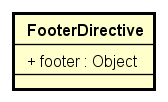
\includegraphics[scale=0.45]{UML/Classi/Front-End/QuizziPedia_Front-end_FooterDirective.png}
	\caption{QuizziPedia::Front-End::Views:FooterDirective}
\end{figure} \FloatBarrier
\begin{itemize}
	\item \textbf{Descrizione}: directive contenente i componenti grafici del footer dell'applicazione;
	\item \textbf{Utilizzo}: premette di visualizzare le informazioni contenenti nel footer in ogni pagina dell'applicazione;
	\item \textbf{Relazioni con altre classi}:
	\begin{itemize}
		\item \textit{IN} \texttt{Index}: contenitore generale dell'applicazione.
	\end{itemize}
	\item \textbf{Attributi}:
	\begin{itemize}
		\item {+ footer: Object} \\ Oggetto contenente le informazioni presenti nel footer.
	\end{itemize}
\end{itemize}

\paragraph{QuizziPedia::Front-End::Directives::ImageInTheQuestionDirective}
\begin{figure} [ht]
	\centering
	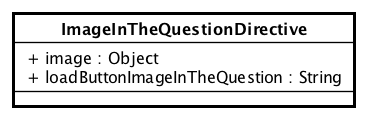
\includegraphics[scale=0.45]{UML/Classi/Front-End/QuizziPedia_Front-end_ImageInTheQuestionDirective.png}
	\caption{QuizziPedia::Front-End::Views:ImageInTheQuestionDirective}
\end{figure} \FloatBarrier
\begin{itemize}
	\item \textbf{Descrizione}: directive contenente i componenti grafici per l'inserimento dell'immagine nella creazione delle domande;
	\item \textbf{Utilizzo}: permette di per inserire un'immagine in una domanda;
	\item \textbf{Relazioni con altre classi}:
	\begin{itemize}
		\item \textit{IN} \texttt{TrueFalseQuestionsView}: view contenente i campi per creare una domanda vero/falso; 
		\item \textit{IN} \texttt{MultipleQuestionsView}:  view contenente i campi per creare una domanda vero/falso; 
		\item \textit{IN} \texttt{ImagesSortingQuestionsView}: view contenente i campi per creare una domanda a ordinamento immagini;
		\item \textit{IN} \texttt{ClickableAreaQuestionsView}:  view contenente i campi per creare una domanda ad area cliccabile.
	\end{itemize}
	\item \textbf{Attributi}:
	\begin{itemize}
		\item {+ image: String} \\ Attributo contenete l'immagine caricata dall'utente;
		\item {+ loadButton: String} \\ Attributo che viene utilizzato per visualizzare la giusta traduzione della \textit{label\ped{G}} per il bottone di caricamento dell'immagine, in italiano o in inglese. 
	\end{itemize}
\end{itemize}